\documentclass{article}
\usepackage[utf8]{inputenc} %кодировка
\usepackage[T2A]{fontenc}
\usepackage[english,russian]{babel} %русификатор 
\usepackage{mathtools} %библиотека матеши
\usepackage[left=1cm,right=1cm,top=2cm,bottom=2cm,bindingoffset=0cm]{geometry} %изменение отступов на листе
\usepackage{amsmath}
\usepackage{graphicx} %библиотека для графики и картинок
\graphicspath{}
\DeclareGraphicsExtensions{.pdf,.png,.jpg}
\usepackage{subcaption}
\usepackage{pgfplots}
\usepackage{float}

\begin{document}
% НАЧАЛО ТИТУЛЬНОГО ЛИСТА
\begin{center}
    \Large
    Федеральное государственное автономное \\
    образовательное учреждение высшего образования \\ 
    «Научно-образовательная корпорация ИТМО»\\
    \vspace{0.5cm}
    \large
    Факультет программной инженерии и компьютерной техники \\
    Направление подготовки 09.03.04 Программная инженерия \\
    \vspace{1cm}
    \Large
    \textbf{Отчёт по лабораторной работе №3} \\
    По дисциплине «Математическая статистика» (4 семестр)\\
    \large
    \vspace{8cm}

    \begin{minipage}{.33\textwidth}
    \end{minipage}
    \hfill
    \begin{minipage}{.4\textwidth}
    
        \textbf{Студент}: \vspace{.1cm} \\
        \ Дениченко Александр P3212\\
        \textbf{Практик}:  \\
        \ Наумова Надежда Александровна
    \end{minipage}
    \vfill
Санкт-Петербург\\ 2024 г.
\end{center}
\pagestyle{empty}
% КОНЕЦ ТИТУЛЬНОГО ЛИСТА 
\newpage
\pagestyle{plain}
\section{Цель работы}
Найти приближенное значение определенного интеграла с требуе-
мой точностью различными численными методами.
\[\text{Вариант} - 8\]
\section{Вычислительная часть}
1. Вычислить интеграл, приведенный в таблице 1, точно.\\
2. Вычислить интеграл по формуле Ньютона – Котеса при n = 6.\\
3. Вычислить интеграл по формулам средних прямоугольников, трапеций и Симпсона при n = 10 .\\
4. Сравнить результаты с точным значением интеграла.\\
5. Определить относительную погрешность вычислений для каждого метода.\\
6. В отчете отразить последовательные вычисления.\\
\\
\textbf{Интеграл по варианту:}
\[\int_{2}^{3}3x^3-2x^2-7x-8\]
\textbf{Точное вычисление интеграла:}
\[\int_{2}^{3}3x^3-2x^2-7x-8 = \left(\frac{3x^4}{4} - \frac{2x^3}{3} - \frac{7x^2}{2}-8x\right)\biggr|_2^3 = \frac{243}{4} - \frac{301}{6} = \frac{127}{12} \approx 10.583\]
\textbf{Вычисление по формуле Ньютона – Котеса:}\\ \\
Берём n=6, тогда коэффициенты Котеса для равноотстоящих узлов:
\[c_6^0 = c_6^6 = \frac{42(b-a)}{840}\]
\[c_6^1 = c_6^5 = \frac{216(b-a)}{840}\]
\[c_6^2 = c_6^4 = \frac{27(b-a)}{840}\]
\[c_6^3= \frac{272(b-a)}{840}\]
Границы известны a=2; b=3:
\[c_6^0 = c_6^6 = \frac{42}{840}\]
\[c_6^1 = c_6^5 = \frac{216}{840}\]
\[c_6^2 = c_6^4 = \frac{27}{840}\]
\[c_6^3= \frac{272}{840}\]
Найдём шаг разбиения:
\[h = \frac{3-2}{6} = \frac{1}{6}\]
Запишем определенный интеграл в виде:
\[\int_{2}^{3}3x^3-2x^2-7x-8 = c_6^0\cdot f(a) 
+ c_6^1\cdot f(a+\frac{1}{6})
+ c_6^2\cdot f(a+\frac{2}{6}) 
+ c_6^3\cdot f(a+\frac{3}{6})
+ c_6^4\cdot f(a+\frac{4}{6})
+ c_6^5\cdot f(a+\frac{5}{6})
+ c_6^6\cdot f(b)=
\]
\[= \frac{42}{840}\cdot f(2) 
+ \frac{216}{840}\cdot f(2+\frac{1}{6})
+ \frac{27}{840}\cdot f(2+\frac{2}{6}) 
+ \frac{272}{840}\cdot f(2+\frac{3}{6})
+ \frac{27}{840}\cdot f(2+\frac{4}{6})
+ \frac{216}{840}\cdot f(2+\frac{5}{6})
+ \frac{42}{840}\cdot f(3)\approx 10.617
\]
Относительная погрешность:
\[\epsilon = \frac{|10.617 - 10.583|}{10.583}\cdot 100 = 0.32\%\]
\\
\textbf{Вычисление по формуле прямоугольников со средними высотами:}\\ \\
По условия дано n = 10, тогда делим отрезок интегрирования на 10 равных частей по формуле:
\[h=\frac{b-a}{n} = \frac{3-2}{10} = 0.1\]
По формуле средних прямоугольников:
\[I = h\sum_{i=1}^{n}y_{i-\frac{1}{2}}\]
\begin{table}[H]
    \centering
    \begin{tabular}{|c|c|c|c|c|c|c|c|c|c|c|c|}
        \hline
        $i$ & 0 & 1 & 2 & 3 & 4 & 5 & 6& 7& 8& 9& 10\\
        \hline
        $x_i$ & 2 & 2,1 & 2,2& 2,3& 2,4& 2,5& 2,6& 2,7& 2,8& 2,9& 3\\
        \hline
        $y_i$ &-6& -3.737& -1.136& 1.821& 5.152& 8.875& 13.008& 17.569& 22.576& 28.047& 34 \\
        \hline
        $x_{i-1/2}$ & & 2.05 & 2.15 & 2.25 & 2.35 & 2.45& 2.55& 2.65& 2.75& 2.85& 2.95 \\
        \hline
        $y_{i-1/2}$ & & -4.9096& -2.4799& 0.2969& 3.4386& 6.9634& 10.8891& 15.2339& 20.0156& 25.2524& 30.9621 \\
        \hline
        \end{tabular}
        \caption{Приближенное вычисление интеграла методом средних прямоугольников}
        \label{tab:midpoint_approximation}  
\end{table}
Подсчёт:
\[I = 0.1\cdot (-4.9096 -2.4799+ 0.2969+ 3.4386+ 6.9634+ 10.8891+ 15.2339+ 20.0156+ 25.2524+ 30.9621) = 10.8737\]
Относительная погрешность:
\[\epsilon = \frac{|10.8737 - 10.583|}{10.583}\cdot 100 = 2.75\%\]
\\
\textbf{Вычисление методом трапеций:}\\ \\
По условия дано n = 10, тогда делим отрезок интегрирования на 10 равных частей по формуле:
\[h=\frac{b-a}{n} = \frac{3-2}{10} = 0.1\]
По формуле трапеций:
\[I = h\cdot \left(\frac{y_0+y_{10}}{2}+\sum_{i=1}^{n-1}y_i\right)\]
\begin{table}[H]
    \centering
    \begin{tabular}{|c|c|c|c|c|c|c|c|c|c|c|c|}
        \hline
        $i$ & 0 & 1 & 2 & 3 & 4 & 5 & 6& 7& 8& 9& 10\\
        \hline
        $x_i$ & 2 & 2,1 & 2,2& 2,3& 2,4& 2,5& 2,6& 2,7& 2,8& 2,9& 3\\
        \hline
        $y_i$ &-6& -3.737& -1.136& 1.821& 5.152& 8.875& 13.008& 17.569& 22.576& 28.047& 34 \\
        \hline
        \end{tabular}
        \caption{Приближенное вычисление интеграла методом трапеций}
        \label{tab:midpoint_approximation}  
\end{table}
Подсчёт:
\[I = 0.1\cdot \left(\frac{-6+43}{2}+(-6-3.737-1.136+1.821+5.152+8.875+13.008+17.569+22.576 +28.047)\right) = 10.0175\]
Относительная погрешность:
\[\epsilon = \frac{|10.0175 - 10.583|}{10.583}\cdot 100 = 5.34\%\]
\\
\textbf{Вычисление методом Симпсона:}\\ \\
По условия дано n = 10, тогда делим отрезок интегрирования на 10 равных частей по формуле:
\[h=\frac{b-a}{n} = \frac{3-2}{10} = 0.1\]
По формуле Симпсона:
\[I = \frac{h}{3}(y_0+ 4\cdot(y_1 + y_3+ y_5+ y_7+ y_9)+2\cdot(y_2 + y_4+ y_6+ y_8) + y_{10}) = \] 
\begin{table}[H]
    \centering
    \begin{tabular}{|c|c|c|c|c|c|c|c|c|c|c|c|}
        \hline
        $i$ & 0 & 1 & 2 & 3 & 4 & 5 & 6& 7& 8& 9& 10\\
        \hline
        $x_i$ & 2 & 2,1 & 2,2& 2,3& 2,4& 2,5& 2,6& 2,7& 2,8& 2,9& 3\\
        \hline
        $y_i$ &-6& -3.737& -1.136& 1.821& 5.152& 8.875& 13.008& 17.569& 22.576& 28.047& 34 \\
        \hline
        \end{tabular}
        \caption{Приближенное вычисление интеграла методом Симпсона}
        \label{tab:midpoint_approximation}  
\end{table}

\[= \frac{0.1}{3}(-6+ 4\cdot(-3.737 + 1.821+ 8.875+ 17.569+ 28.047)+2(-1.136 + 5.152+ 13.008+ 22.576) + 34) = 10.5833\]\\
Относительная погрешность:
\[\epsilon = \frac{|10.5833 - 10.583|}{10.583}\cdot 100 = 0.0028\%\]
\\
\end{document}
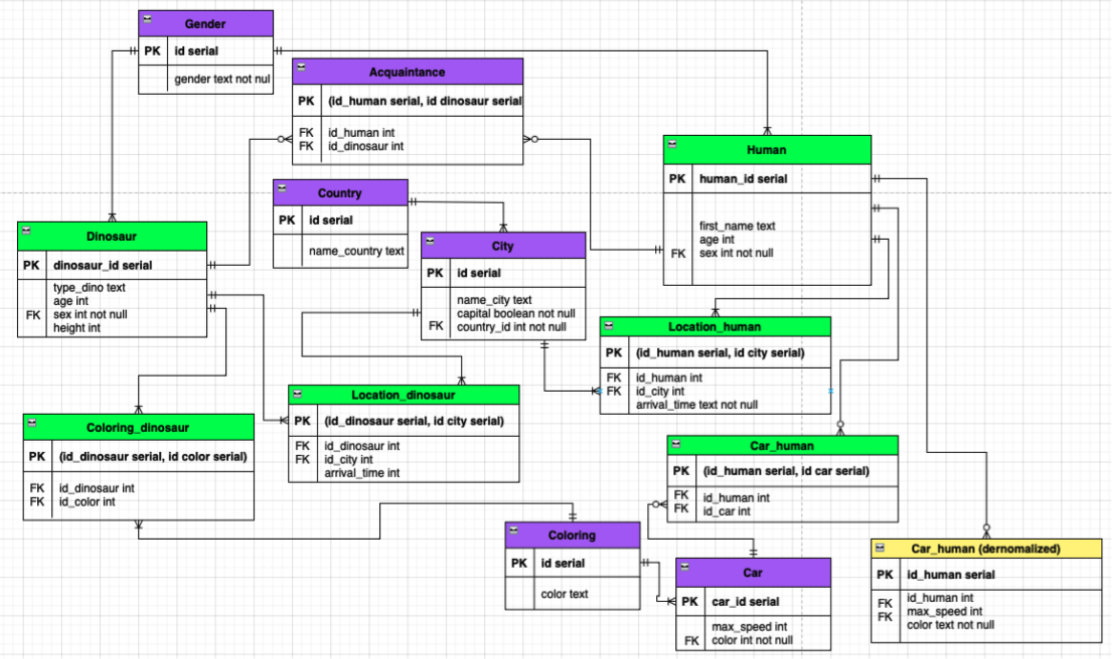
\includegraphics[width=.9\textwidth]{123}